\documentclass[12pt,leqno]{article}
\usepackage[left=1in,top=1in,right=1in,bottom=1in]{geometry}
\newcommand*{\authorfont}{\fontfamily{phv}\selectfont}
\usepackage{lmodern}


  \usepackage[T1]{fontenc}




\usepackage{abstract}
\renewcommand{\abstractname}{}    % clear the title
\renewcommand{\absnamepos}{empty} % originally center

\renewenvironment{abstract}
 {{%
    \setlength{\leftmargin}{0mm}
    \setlength{\rightmargin}{\leftmargin}%
  }%
  \relax}
 {\endlist}

\makeatletter
\def\@maketitle{%
  \newpage
%  \null
%  \vskip 2em%
%  \begin{center}%
  \let \footnote \thanks
    {\fontsize{18}{20}\selectfont\raggedright  \setlength{\parindent}{0pt} \@title \par}%
}
%\fi
\makeatother




\setcounter{secnumdepth}{0}



\title{Day 05: Consistency, Precision and Neymanian Hypothesis Tests  }



\author{\Large \href{mailto:t.leavitt718@gmail.com}{Thomas Leavitt}\vspace{0.05in} \newline\normalsize\emph{}  }


\date{}

\usepackage{titlesec}

\titleformat*{\section}{\normalsize\bfseries}
\titleformat*{\subsection}{\normalsize\itshape}
\titleformat*{\subsubsection}{\normalsize\itshape}
\titleformat*{\paragraph}{\normalsize\itshape}
\titleformat*{\subparagraph}{\normalsize\itshape}


\usepackage{natbib}
\bibliographystyle{apsr}



\newtheorem{hypothesis}{Hypothesis}
\usepackage{setspace}

\makeatletter
\@ifpackageloaded{hyperref}{}{%
\ifxetex
  \usepackage[setpagesize=false, % page size defined by xetex
              unicode=false, % unicode breaks when used with xetex
              xetex]{hyperref}
\else
  \usepackage[unicode=true]{hyperref}
\fi
}
\@ifpackageloaded{xcolor}{
    \PassOptionsToPackage{usenames,dvipsnames}{xcolor}
}{%
    \usepackage[usenames,dvipsnames]{xcolor}
}
\makeatother
\hypersetup{breaklinks=true,
            bookmarks=true,
            pdfauthor={\href{mailto:t.leavitt718@gmail.com}{Thomas Leavitt} ()},
             pdfkeywords = {},  
            pdftitle={Day 05: Consistency, Precision and Neymanian Hypothesis Tests},
            colorlinks=true,
            citecolor=blue,
            urlcolor=blue,
            linkcolor=magenta,
            pdfborder={0 0 0}}
\urlstyle{same}  % don't use monospace font for urls

% \usepackage{microtype} %
% \usepackage{setspace}
% \onehalfspacing
\usepackage{xcolor, color, ucs}     % http://ctan.org/pkg/xcolor
\usepackage{natbib}
\usepackage{booktabs}          % package for thick lines in tables
\usepackage{amsfonts,amsthm,amsmath,amssymb,bm}          % AMS Fonts
% \usepackage{empheq}            % To use left brace on {align} environment
\usepackage{graphicx}          % Insert .pdf, .eps or .png
\usepackage{enumitem}          % http://ctan.org/pkg/enumitem
% \usepackage[mathscr]{euscript}          % Font for right expectation sign
\usepackage{tabularx}          % Get scale boxes for tables
\usepackage{float}             % Force floats around
\usepackage{rotating}          % Rotate long tables horizontally
\usepackage{bbm}                % for bold betas
\usepackage{csquotes}           % \enquote{} and \textquote[][]{} environments
\usepackage{subfigure}
\usepackage{array}
% \usepackage{cancel}
\usepackage{longtable}
% % \usepackage{lmodern}
% % \usepackage{libertine} \usepackage[libertine]{newtxmath}
% \usepackage{stix}
% % \usepackage[osf,sc]{mathpazo}     % alternative math
% \usepackage[T1]{fontenc}
% \usepackage{fontspec}
% \setmainfont{Times New Roman}
% \usepackage{mathtools}          % multlined environment with size option
% \usepackage{verbatim}
% \usepackage{geometry}
% \usepackage{bigfoot}
% \geometry{verbose,margin=.8in,nomarginpar}
% \setcounter{secnumdepth}{2}
% \setcounter{tocdepth}{2}
% \usepackage{lscape}

\setlist{nosep}


% \usepackage{url}
% \usepackage[nobreak=true]{mdframed} % put box around section with \begin{mdframed}\end{mdframed}

% \usepackage{relsize}            % \mathlarger{} environment
% \usepackage[unicode=true,
%             pdfusetitle,
%             bookmarks=true,
%             bookmarksnumbered=true,
%             bookmarksopen=true,
%             bookmarksopenlevel=2,
%             breaklinks=false,
%             pdfborder={0 0 1},
%             backref=false,
%             colorlinks=true,
%             hypertexnames=false]{hyperref}
% \hypersetup{pdfstartview={XYZ null null 1},
%             citecolor=blue!50,
%             linkcolor=red,
%             urlcolor=green!70!black}

% \usepackage{multirow}
% \usepackage{tikz}
% \usetikzlibrary{trees, positioning, arrows, automata}

% \tikzset{
%   treenode/.style = {align=center, inner sep=0pt, text centered,
%     font=\sffamily},
%   arn_n/.style = {treenode, rectangle, black, fill=white, text width=6em},
%   arn_r/.style = {treenode, circle, red, draw=red, text width=1.5em, thick}
% }

\usepackage[noabbrev]{cleveref} % Should be loaded after \usepackage{hyperref}
\usepackage[small,bf]{caption}  % Captions

% \usepackage[obeyFinal,textwidth=0.8in, colorinlistoftodos,prependcaption,textsize=tiny]{todonotes} % \fxnote*[options]{note}{text} to make sticky notes
% \usepackage{xargs}
% \newcommandx{\unsure}[2][1=]{\todo[linecolor=red,backgroundcolor=red!25,bordercolor=red,#1]{#2}}
% \newcommandx{\change}[2][1=]{\todo[linecolor=blue,backgroundcolor=blue!25,bordercolor=blue,#1]{#2}}
% \newcommandx{\info}[2][1=]{\todo[linecolor=OliveGreen,backgroundcolor=OliveGreen!25,bordercolor=OliveGreen,#1]{#2}}
% \newcommandx{\improvement}[2][1=]{\todo[linecolor=Plum,backgroundcolor=Plum!25,bordercolor=Plum,#1]{#2}}

\parskip=8pt
\parindent=0pt
\delimitershortfall=-1pt
\interfootnotelinepenalty=100000

\newcommand{\qedknitr}{\hfill\rule{1.2ex}{1.2ex}}

% \makeatletter
% \def\thm@space@setup{\thm@preskip=0pt
% \thm@postskip=0pt}
% \makeatother

\def\tightlist{}

\makeatletter
% align all math after the command
\newcommand{\mathleft}{\@fleqntrue\@mathmargin\parindent}
\newcommand{\mathcenter}{\@fleqnfalse}
% tilde with text over it
\newcommand{\distas}[1]{\mathbin{\overset{#1}{\kern\z@\sim}}}%
\newsavebox{\mybox}\newsavebox{\mysim}
\newcommand{\distras}[1]{%
  \savebox{\mybox}{\hbox{\kern3pt$\scriptstyle#1$\kern3pt}}%
  \savebox{\mysim}{\hbox{$\sim$}}%
  \mathbin{\overset{#1}{\kern\z@\resizebox{\wd\mybox}{\ht\mysim}{$\sim$}}}%
}
\makeatother

% \newtheoremstyle{newstyle}
% {} %Aboveskip
% {} %Below skip
% {\mdseries} %Body font e.g.\mdseries,\bfseries,\scshape,\itshape
% {} %Indent
% {\bfseries} %Head font e.g.\bfseries,\scshape,\itshape
% {.} %Punctuation afer theorem header
% { } %Space after theorem header
% {} %Heading

\theoremstyle{newstyle}
\newtheorem{thm}{Theorem}
\newtheorem{prop}[thm]{Proposition}
\newtheorem{lem}{Lemma}
\newtheorem{cor}{Corollary}
\newtheorem{definition}{Definition}
\newcommand*\diff{\mathop{}\!\mathrm{d}}
\newcommand*\Diff[1]{\mathop{}\!\mathrm{d^#1}}
\DeclareMathOperator{\E}{\mathbb{E}}
\DeclareMathOperator{\R}{\mathbb{R}}
\newcolumntype{L}[1]{>{\raggedright\let\newline\\\arraybackslash\hspace{0pt}}m{#1}}
\newcolumntype{C}[1]{>{\centering\let\newline\\\arraybackslash\hspace{0pt}}m{#1}}
\newcolumntype{R}[1]{>{\raggedleft\let\newline\\\arraybackslash\hspace{0pt}}m{#1}}

% suppress table numbering
\captionsetup[table]{labelformat=empty}


\begin{document}
	
% \pagenumbering{arabic}% resets `page` counter to 1 
%
% \maketitle

{% \usefont{T1}{pnc}{m}{n}
\setlength{\parindent}{0pt}
\thispagestyle{plain}
{\fontsize{18}{20}\selectfont\raggedright 
\maketitle  % title \par  

}

{
   \vskip 13.5pt\relax \normalsize\fontsize{11}{12} 
\textbf{\authorfont \href{mailto:t.leavitt718@gmail.com}{Thomas Leavitt}} \hskip 15pt \emph{\small }   

}

}





\vskip 6.5pt

\noindent  \hypertarget{consistency}{%
\section{Consistency}\label{consistency}}

We demonstrate our arguments via a simple hypothetical example that
consists of \(n = 6\) units and an individual assignment process
(complete, individual assignment) in which \(3\) units are assigned to
treatment (\(n_1 = 3\)) and to control (\(n_0 = 3\)). Let's further
imagine that (unbeknownst to the researcher) the \(6\) units' potential
outcomes and individual causal effects are as follows in
\cref{tab: true potential outcomes}:

\begin{table}[H]
\centering{}
    \begin{tabular}{l|l|l}
    $\mathbf{y_c}$ & $\mathbf{y_t}$ & $\pmb{\tau}$ \\ \midrule
    20 & 22 & 2 \\
     8 & 12 & 4 \\
    11 & 11 & 0 \\
    10 & 15 & 5 \\
    14 & 18 & 4 \\
     1 &  4 & 3 \\
    \end{tabular}
\caption{True values of $\mathbf{y_c}$, $\mathbf{y_t}$ and $\pmb{\tau}$, where $\tau_i = y_{t,i} - y_{c,i}$, for the study population} \label{tab: true potential outcomes}
\end{table}

Based on the complete, individual assignment process in which there are
\(n = 6\) units and \(n_1 = 3\) of which are assigned to treatment, the
set of \(\left\lvert \Omega \right\rvert = \binom{6}{3} = 20\) possible
assignments is given by \cref{eq: example omega}: \begin{equation}
\Omega =
\left\{
\begin{bmatrix} 1 \\ 1 \\ 1 \\ 0 \\ 0 \\ 0 \end{bmatrix},
\begin{bmatrix} 1 \\ 1 \\ 0 \\ 1 \\ 0 \\ 0 \end{bmatrix},
%\begin{bmatrix} 1 \\ 1 \\ 0 \\ 0 \\ 1 \\ 0 \end{bmatrix},
%\begin{bmatrix} 1 \\ 1 \\ 0 \\ 0 \\ 0 \\ 1 \end{bmatrix},
%\begin{bmatrix} 1 \\ 0 \\ 1 \\ 1 \\ 0 \\ 0 \end{bmatrix},
%\begin{bmatrix} 1 \\ 0 \\ 1 \\ 0 \\ 1 \\ 0 \end{bmatrix},
%\begin{bmatrix} 1 \\ 0 \\ 1 \\ 0 \\ 0 \\ 1 \end{bmatrix},
%\begin{bmatrix} 1 \\ 0 \\ 0 \\ 1 \\ 1 \\ 0 \end{bmatrix},
%\begin{bmatrix} 1 \\ 0 \\ 0 \\ 1 \\ 0 \\ 1 \end{bmatrix},
%\begin{bmatrix} 1 \\ 0 \\ 0 \\ 0 \\ 1 \\ 1 \end{bmatrix},
%\begin{bmatrix} 0 \\ 1 \\ 1 \\ 1 \\ 0 \\ 0 \end{bmatrix},
%begin{bmatrix} 0 \\ 1 \\ 1 \\ 0 \\ 1 \\ 0 \end{bmatrix},
%\begin{bmatrix} 0 \\ 1 \\ 1 \\ 0 \\ 0 \\ 1 \end{bmatrix},
%\begin{bmatrix} 0 \\ 1 \\ 0 \\ 1 \\ 1 \\ 0 \end{bmatrix},
%\begin{bmatrix} 0 \\ 1 \\ 0 \\ 1 \\ 0 \\ 1 \end{bmatrix},
%\begin{bmatrix} 0 \\ 1 \\ 0 \\ 0 \\ 1 \\ 1 \end{bmatrix},
%\begin{bmatrix} 0 \\ 0 \\ 1 \\ 1 \\ 1 \\ 0 \end{bmatrix},
%\begin{bmatrix} 0 \\ 0 \\ 1 \\ 1 \\ 0 \\ 1 \end{bmatrix},
\cdots,
\begin{bmatrix} 0 \\ 0 \\ 1 \\ 0 \\ 1 \\ 1 \end{bmatrix},
\begin{bmatrix} 0 \\ 0 \\ 0 \\ 1 \\ 1 \\ 1 \end{bmatrix}
\right\}.
\label{eq: example omega}
\end{equation}

The assignment one draws from the set \(\Omega\) determines which
potential outcomes one observes. One can observe treatment potential
outcomes only for units assigned to treatment and control potential
outcomes only for units assigned to control. (Recall the function
\(y_i = z_iy_{t,i} + \left(1 - z_i\right)y_{c,i}\), which determines the
potential outcome one observes for each individual \(i\).) As Table
\ref{tab: outcomes of experiment} shows, for each of the
\(\binom{6}{3} = 20\) possible assignments, there are
\(\binom{6}{3} = 20\) corresponding possible realizations of observed
data \(y\):

\begin{table}[H]
\scriptsize
    \begin{tabular}{l|l|l|l|}
    $\mathbf{z}_1$ & $\mathbf{y_c}$ & $\mathbf{y_t}$ & $\mathbf{y}_1$ \\ \midrule
    1 & ?  & 22  & 22 \\
    1 & ?  & 12  & 12 \\
    1 & ?  & 11  & 11 \\
    0 & 10 & ?   & 10 \\
    0 & 14 & ?   & 14 \\
    0 &  1 & ?   &  1 \\
    \end{tabular}
    \hfill
      \begin{tabular}{l|l|l|l|}
    $\mathbf{z}_2$ & $\mathbf{y_c}$ & $\mathbf{y_t}$ & $\mathbf{y}_2$ \\ \midrule
    1 &  ? & 22 & 22 \\
    1 &  ? & 12 & 12 \\
    0 & 11 & ?  & 11 \\
    1 & ?  & 15 & 15 \\
    0 & 14 & ?  & 14 \\
    0 &  1 & ?  &  1 \\
    \end{tabular}
     \hfill
     $\cdots $
     \hfill
      \begin{tabular}{l|l|l|l|}
    $\mathbf{z}_{19}$ & $\mathbf{y_c}$ & $\mathbf{y_t}$ & $\mathbf{y}_{19}$ \\ \midrule
    0 & 20 & ?  & 20 \\
    0 &  8 & ?  &  8 \\
    1 &  ? & 11 & 11 \\
    0 & 10 & ?  & 10 \\
    1 & ?  & 18 & 18 \\
    1 & ?  &  4 &  4 \\
    \end{tabular}
     \hfill
      \begin{tabular}{l|l|l|l|}
    $\mathbf{z}_{20}$ & $\mathbf{y_c}$ & $\mathbf{y_t}$ & $\mathbf{y}_{20}$ \\ \midrule
    0 & 20 & ?  & 20 \\
    0 &  8 & ?  &  8 \\
    0 & 11 & ?  & 11 \\
    1 & ?  & 15 & 15 \\
    1 & ?  & 18 & 18 \\
    1 & ?  &  4 &  4 \\
    \end{tabular}
    \caption{All possible realizations of experimental data from a completely randomized study with 6 units and 3 treated units.}
\label{tab: outcomes of experiment}
\end{table}

If we have an experimental pool of 6 units, that are not a sample using
a known procedure from a well-defined population, what does
\enquote{asymptotic growth} mean? We follow \citet{brewer1979} and
\citet{middletonaronow2015} in using the idea of \enquote{copies} as a
way to talk about how estimators and tests behave as study sizes
increase. In short, this conception of asymptotic growth states that (1)
the original population of \(n\) units is copied \(h - 1\) times; (2)
within each of the \(h\) copies, exactly \(n_1\) units are assigned to
the treatment condition and the remaining \(n_0 = n - n_1\) units are
assigned to the control condition; (3) the \(h\) copies are then
collected into a single population with \(h n\) total units, \(h n_1\)
treated units and \(h n_0\) control units.

In the context of our working example, this conception of growth
stipulates that the study population of \(N = 6\) units is embedded in a
sequence of populations of increasing sizes in which the initial
population is simply copied \(h - 1\) times:

\begin{table}[H]
\scriptsize
\centering
\begin{tabular}{l|l|l}
$\mathbf{y_c}$ & $\mathbf{y_t}$ & $\pmb{\tau}$ \\ \midrule
20 & 22 &  2 \\
8  & 12 &  4 \\
11 & 11 &  0 \\
10 & 15 &  5 \\
14 & 18 &  4 \\
1  &  4 &  3
\end{tabular}
\hfill
\begin{tabular}{l|l|l}
$\mathbf{y_c}$ & $\mathbf{y_t}$ & $\pmb{\tau}$ \\ \midrule
20 & 22 &  2 \\
8  & 12 &  4 \\
11 & 11 &  0 \\
10 & 15 &  5 \\
14 & 18 &  4 \\
1  &  4 &  3 \\ \midrule
20 & 22 &  2 \\
8  & 12 &  4 \\
11 & 11 &  0 \\
10 & 15 &  5 \\
14 & 18 &  4 \\
1  &  4 &  3
\end{tabular}
\hfill
\begin{tabular}{l|l|l}
$\mathbf{y_c}$ & $\mathbf{y_t}$ & $\pmb{\tau}$ \\ \midrule
20 & 22 &  2 \\
8  & 12 &  4 \\
11 & 11 &  0 \\
10 & 15 &  5 \\
14 & 18 &  4 \\
1  &  4 &  3 \\ \midrule
20 & 22 &  2 \\
8  & 12 &  4 \\
11 & 11 &  0 \\
10 & 15 &  5 \\
14 & 18 &  4 \\
1  &  4 &  3 \\ \midrule
20 & 22 &  2 \\
8  & 12 &  4 \\
11 & 11 &  0 \\
10 & 15 &  5 \\
14 & 18 &  4 \\
1  &  4 &  3
\end{tabular}
\hfill
\begin{tabular}{l|l|l}
$\mathbf{y_c}$ & $\mathbf{y_t}$ & $\pmb{\tau}$ \\ \midrule
20 & 22 &  2 \\
8  & 12 &  4 \\
11 & 11 &  0 \\
10 & 15 &  5 \\
14 & 18 &  4 \\
1  &  4 &  3 \\ \midrule
20 & 22 &  2 \\
8  & 12 &  4 \\
11 & 11 &  0 \\
10 & 15 &  5 \\
14 & 18 &  4 \\
1  &  4 &  3 \\ \midrule
20 & 22 &  2 \\
8  & 12 &  4 \\
11 & 11 &  0 \\
10 & 15 &  5 \\
14 & 18 &  4 \\
1  &  4 &  3 \\ \midrule
20 & 22 &  2 \\
8  & 12 &  4 \\
11 & 11 &  0 \\
10 & 15 &  5 \\
14 & 18 &  4 \\
1  &  4 &  3
\end{tabular}
$\cdots$
\caption{Finite populations under asymptotic growth in which $h \in \left\{1, 2, 3, 4, \ldots \right\}$}
\label{tab: asymp growth}
\end{table}

Notice that over this sequence of increasing finite populations in Table
\ref{tab: asymp growth}, all relevant factors other than \(N\) remain
constant: The proportions of treatment and control units remain fixed,
the mean of control and treatment potential outcomes remain fixed, as do
their variances and their covariance. Notice, however, that the number
of possible assignments increases over this sequence of increasing
finite populations from \(\binom{6}{3} = 20\) to \(\binom{12}{6} = 924\)
to \(\binom{18}{9} = 48620\) to \(\binom{24}{12} = 2704156\) and so
forth.

In contrast to unbiasedness, consistency states that as the number of
units in the study grows asymptotically, holding all other factors
constant, the probability of an estimate within an arbitrarily small
distance, \(\varepsilon\), from the truth is equal to \(1\). More
formally, we can define consistency as follows: \begin{equation}
\lim_{h \to \infty} \Pr\left(\left\lvert \hat{\bar{\tau}}\left(\mathbf{Z}, \mathbf{Y}\right) - \bar{\tau} \right\rvert < \varepsilon \right) = 1 \text{ for all } \varepsilon > 0
\label{eq: consistency I}
\end{equation} or equivalently as \begin{equation}
\lim_{h \to \infty} \Pr\left(\hat{\bar{\tau}}\left(\mathbf{Z}, \mathbf{Y}\right) \in \left(\bar{\tau} - \varepsilon, \bar{\tau} + \varepsilon\right)\right) = 1 \text{ for all } \varepsilon > 0,
\label{eq: consistency II}
\end{equation} where, referring back to the conception of asymptotic
growth in Table \ref{tab: asymp growth}, \(h\) is the number of copies
of the original finite population from Table
\ref{tab: true potential outcomes}.

To unpack Equations \ref{eq: consistency I} and
\ref{eq: consistency II}, Figure \ref{fig: asymp dists diff-means est}
shows what happens to the distribution of the Difference-in-Means
estimator under complete random assignment as \(h \to \infty\):

\begin{figure}[H]
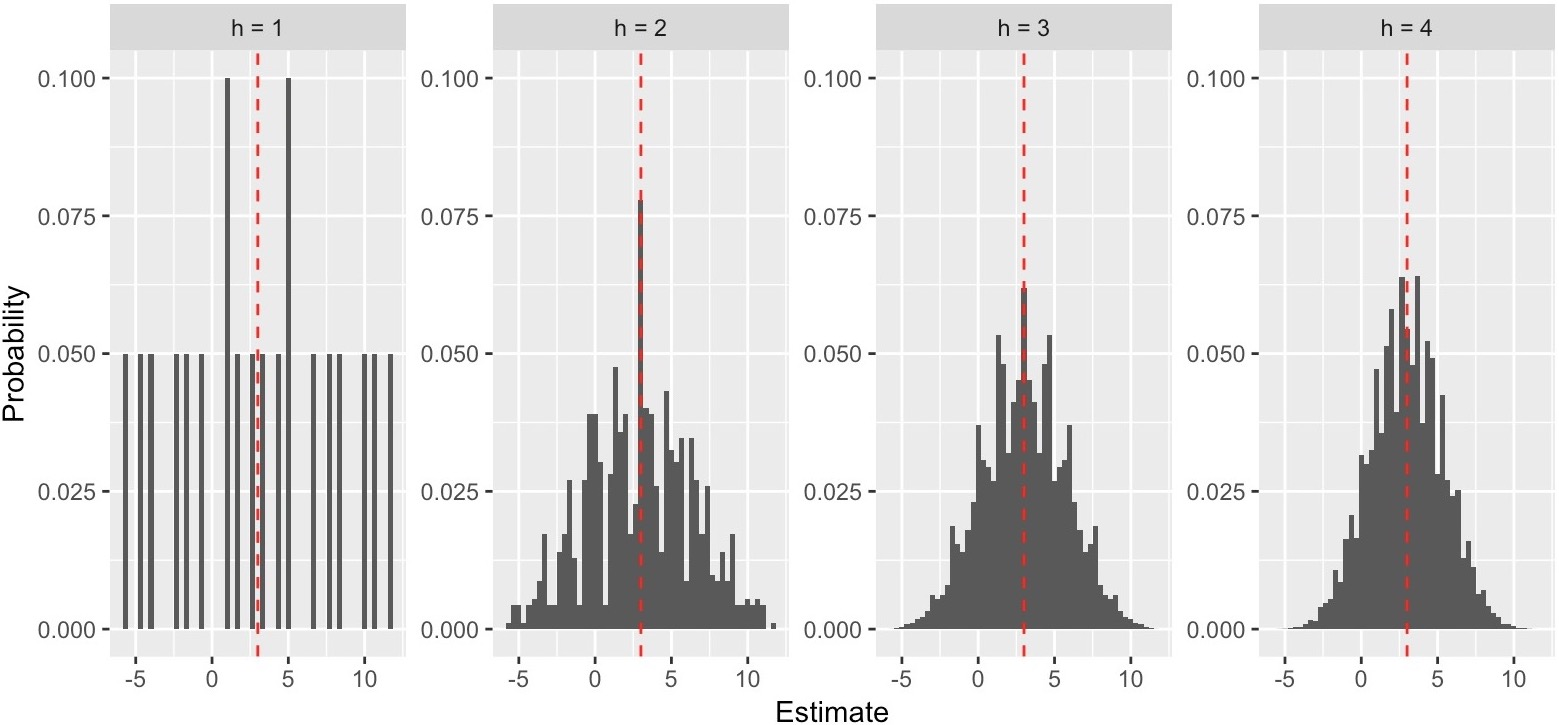
\includegraphics[width=\linewidth]{asymp_ests_plot.jpg}
\caption{Distribution of Difference-in-Means estimator as $h \to \infty$}
\label{fig: asymp dists diff-means est}
\end{figure}

The general trend is that the probability of estimates close to the true
mean causal effect, \(\bar{\tau} = 3\), grows larger and larger and
ultimately converge in probability (over the sequence of increasing
finite populations) to \(1\). For example, following
\cref{eq: consistency II}, consider the probability that an estimate
lies on the interval \(\left(3 - \varepsilon, 3 + \varepsilon \right)\)
and let \(\varepsilon = 1\). The respective probabilities of an estimate
on this interval for \(h \in \left\{1, 2, 3, 4\right\}\) are \(0.1\),
\(0.2359\), \(0.2559\) and \(0.2994\), and as \(h \to \infty\) that
probability tends to \(1\). This property holds for \(\varepsilon = 1\)
as well as for any positive value of \(\varepsilon\) that one could
choose. For example, we could have let \(\varepsilon = 0.5\), in which
case the corresponding probabilities for
\(h \in \left\{1, 2, 3, 4\right\}\) are \(0.1\), \(0.1234\), \(0.1522\)
and \(0.1643\), and the limiting probability as \(h \to \infty\) is also
\(1\).

\section{Precision}

\citet{neyman1923} derived an exact analytic expression for the variance
of the Difference-in-Means estimator based solely on the research design
of a randomized experiment as follows: \begin{equation}
\sigma^2_{\hat{\bar{\tau}}} = \frac{1}{N - 1}\left(\frac{n_1 \sigma^2_{y_c}}{n_0} + \frac{\left(N - n_1\right) \sigma^2_{y_t}}{n_1} + 2\sigma_{y_c, y_t}\right),
\label{eq: var}
\end{equation} where \(\sigma^2_{y_c}\) is the variance of control
potential outcomes, \(\sigma^2_{y_t}\) is the variance of treated
potential outcomes and \(\sigma_{y_c, y_t}\) is the covariance of
control and treated potential outcomes.

As the components marked in \textcolor{red}{red} \textit{increase},
while all other components are held constant, the standard error
\textit{decreases}. By contrast, as the components marked in
\textcolor{blue}{blue} \textit{increase}, while all other components are
held constant, the standard error \textit{increases}:

\begin{equation*}
\sigma^2_{\hat{\bar{\tau}}} = \frac{1}{\textcolor{red}{n} - 1}\left(\frac{n_1 \textcolor{blue}{\sigma^2_{y_c}}}{\left(n - n_1\right)} + \frac{\left(n - n_1\right) \textcolor{blue}{\sigma^2_{y_t}}}{n_1} + 2\textcolor{blue}{\sigma_{y_c, y_t}}\right)
\end{equation*}

Three implications of equation \eqref{eq: var}, as
\citet[58]{gerbergreen2012} state, are:

\begin{itemize}
\item If $\sigma^2_{y_t} > \sigma^2_{y_c}$, then adding additional units to the treatment condition lowers the standard error. 

\item By contrast, if $\sigma^2_{y_t} < \sigma^2_{y_c}$ , then adding more units to the control condition lowers the standard error. 

\item Finally, if $\sigma^2_{y_t} \approx \sigma^2_{y_t}$, then assigning roughly half of subjects to each condition is best for lowering the standard error.
\end{itemize}

\subsection{Estimating the Variance}

The analytic expression for the variance of the difference-in-means
estimator is as follows: \begin{equation*}
\sigma^2_{\hat{\theta}} = \frac{1}{n - 1}\left(\frac{n_1 \sigma^2_{y_c}}{\left(n - n_1\right)} + \frac{\left(n - n_1\right) \sigma^2_{y_t}}{n_1} + 2\sigma_{y_c, y_t}\right),
\end{equation*} where \(\sigma^2_{y_c}\) is the variance of control
potential outcomes, \(\sigma^2_{y_t}\) is the variance of treated
potential outcomes and \(\sigma_{y_c, y_t}\) is the covariance of
control and treated potential outcomes.

The covariance of potential outcomes, \(\sigma_{y_c, y_t}\), is defined
as follows: \begin{equation*}
\begin{split}
\sigma_{y_c, y_t} & \equiv \left(\frac{1}{N}\right) \sum \limits_{i = 1}^N \left(y_{c_i} - \mu_{y_c}\right)\left(y_{t_i} - \mu_{y_t}\right) \\
& \equiv \left(\frac{1}{N}\right) \sum \limits_{i = 1}^N y_{c_i} y_{t_i} - y_{c_i}\mu_{y_t} - \mu_{y_c}y_{t_i} + \mu_{y_c}\mu_{y_t} \\
& \equiv \left(\frac{1}{N}\right) \sum \limits_{i = 1}^N y_{c_i} y_{t_i} - \left(\frac{1}{N}\right) \sum \limits_{i = 1}^N y_{c_i}\mu_{y_t} - \left(\frac{1}{N}\right) \sum \limits_{i = 1}^N \mu_{y_c}y_{t_i} + \left(\frac{1}{N}\right) \sum \limits_{i = 1}^N \mu_{y_c}\mu_{y_t} \\
& \equiv \left(\frac{1}{N}\right) \sum \limits_{i = 1}^N y_{c_i} y_{t_i} - \mu_{y_t} \left(\frac{1}{N}\right) \sum \limits_{i = 1}^N y_{c_i} - \mu_{y_c}\left(\frac{1}{N}\right) \sum \limits_{i = 1}^N y_{t_i} + \mu_{y_c}\mu_{y_t} \\ 
& \equiv \left(\frac{1}{N}\right) \sum \limits_{i = 1}^N y_{c_i} y_{t_i} - \mu_{y_t} \mu_{y_c} - \mu_{y_c}\mu_{y_t} + \mu_{y_c}\mu_{y_t} \\ 
& \equiv \underbrace{\left(\frac{1}{N}\right) \sum \limits_{i = 1}^N y_{c_i} y_{t_i}}_{\text{inestimable}} - \underbrace{\mu_{y_t} \mu_{y_c}}_{\text{estimable}}
\end{split}
\end{equation*} We can estimate \(\mu_{y_c}\) and \(\mu_{y_t}\) without
bias, but we cannot estimate
\(\left(\frac{1}{N}\right) \sum \limits_{i = 1}^N y_{c_i} y_{t_i}\)
because we can never observe both \(y_{c_i}\) and \(y_{t_i}\) for any of
the \(i \in \left\{1, \dots , n\right\}\) units.

We can now derive an unbiased or conservatively biased estimator of the
standard error as follows:

By the Cauchy-Schwarz inequality and the inequality of arithmetic and
geometric means
\(2\sigma_{y_c, y_t} \leq \sigma^2_{y_c} + \sigma^2_{y_t}\); hence, if
we substitute \(\sigma^2_{y_c} + \sigma^2_{y_t}\) for
\(2\sigma_{y_c, y_t}\), then the true variance of the
difference-in-means estimator,
\(\frac{1}{n - 1}\left(\frac{n_1 \sigma^2_{y_c}}{\left(n - n_1\right)} + \frac{\left(n - n_1\right) \sigma^2_{y_t}}{n_1} + 2\sigma_{y_c, y_t}\right)\),
is less than or equal to the conservative variance of the
difference-in-means estimator,
\(\frac{1}{n - 1}\left(\frac{n_1 \sigma^2_{y_c}}{\left(n - n_1\right)} + \frac{\left(n - n_1\right) \sigma^2_{y_t}}{n_1} + \sigma^2_{y_c} + \sigma^2_{y_t}\right)\).

We can now substitute \(\sigma^2_{y_c} + \sigma^2_{y_t}\) for
\(2\sigma_{y_c, y_t}\) and further manipulate the conservative variance
expression as follows:

\begin{align*}
\frac{1}{n - 1}\left(\frac{n_1 \sigma^2_{y_c}}{\left(n - n_1\right)} + \frac{\left(n - n_1\right) \sigma^2_{y_t}}{n_1} + 2\sigma_{y_c, y_t}\right)\\
\frac{1}{n - 1}\left(\frac{n_1 \sigma^2_{y_c}}{\left(n - n_1\right)} + \frac{\left(n - n_1\right) \sigma^2_{y_t}}{n_1} + \sigma^2_{y_c} + \sigma^2_{y_t}\right) \\
\frac{1}{n - 1}\left(\frac{n_1 \sigma^2_{y_c}}{\left(n - n_1\right)} + \frac{n\sigma^2_{y_t} - n_1\sigma^2_{y_t}}{n_1} + \sigma^2_{y_c} + \sigma^2_{y_t}\right) \\ 
\frac{1}{n - 1}\left(\frac{n_1 \sigma^2_{y_c}}{\left(n - n_1\right)} + \frac{n\sigma^2_{y_t}}{n_1} - \frac{n_1\sigma^2_{y_t}}{n_1} + \sigma^2_{y_c} + \sigma^2_{y_t}\right) \\
\frac{1}{n - 1}\left(\frac{n_1 \sigma^2_{y_c}}{\left(n - n_1\right)} + \frac{n\sigma^2_{y_t}}{n_1} - \sigma^2_{y_t} + \sigma^2_{y_c} +  \sigma^2_{y_t}\right) \\  
\frac{1}{n - 1}\left(\frac{n_1 \sigma^2_{y_c}}{\left(n - n_1\right)} + \frac{n\sigma^2_{y_t}}{n_1} + \sigma^2_{y_c} \right) \\ 
\frac{1}{n - 1}\left(\frac{n_1 \sigma^2_{y_c}}{\left(n - n_1\right)} + \frac{\left(n - n_1\right)\sigma^2_{y_c}}{\left(n - n_1\right)} + \frac{n\sigma^2_{y_t}}{n_1} \right) \\  
\frac{1}{n - 1}\left(\frac{n_1 \sigma^2_{y_c} + \left(n - n_1\right)\sigma^2_{y_c}}{\left(n - n_1\right)} + \frac{n\sigma^2_{y_t}}{n_1} \right) \\
\frac{1}{n - 1}\left(\frac{n_1 \sigma^2_{y_c} + n\sigma^2_{y_c} - n_1\sigma^2_{y_c}}{\left(n - n_1\right)} + \frac{n\sigma^2_{y_t}}{n_1} \right) \\
\frac{1}{n - 1}\left(\frac{n\sigma^2_{y_c}}{\left(n - n_1\right)} + \frac{n\sigma^2_{y_t}}{n_1} \right) \\
\frac{n}{n - 1}\left(\frac{\sigma^2_{y_c}}{\left(n - n_1\right)} + \frac{\sigma^2_{y_t}}{n_1} \right)  
\end{align*}

The parameters \(\sigma^2_{y_c}\) and \(\sigma^2_{y_t}\) are unknown. We
can, however, ``plug in'' unbiased estimators of these two quantities
for \(\sigma^2_{y_c}\) and \(\sigma^2_{y_t}\). Following
\citet[Theorem 2.4]{cochran1977}, unbiased estimators of
\(\sigma^2_{y_c}\) and \(\sigma^2_{y_t}\), respectively, are:
\(\widehat{\sigma}^2_{y_c} = \left(\frac{n - 1}{n\left(n_0 - 1\right)}\right)\sum \limits_{i: Z_i = 0}^n \left(y_{ci} - \widehat{\mu}_{y_c}\right)^2\)
and
\(\widehat{\sigma}^2_{y_t} = \left(\frac{n - 1}{n\left(n_1 - 1\right)}\right)\sum \limits_{i: Z_i = 1}^{n} \left(y_{ti} - \widehat{\mu}_{y_t}\right)^2\),
where \(n_0 = n - n_1\).

Therefore, the unbiased or conservatively biased estimator of the
variance of the difference-in-means estimator is: \begin{equation*}
\widehat{\sigma}^2_{\hat{\theta}} = \frac{n}{n - 1}\left(\frac{\widehat{\sigma}^2_{y_c}}{\left(n - n_1\right)} + \frac{\widehat{\sigma}^2_{y_t}}{n_1} \right)
\end{equation*}

\section{Neymanian Hypothesis Tests}

Fisherian tests allow the use of many different kinds of test
statistics, Neymanian hypothesis tests are much more closely related to
the estimation of mean causal effects. In any given study, one can
observe only a single \textit{estimate}. However, a researcher can
postulate (provisionally for the sake of argument) a weak null
hypothesis, \(H_0: \bar{\tau} = \bar{\tau}_0\), relative to some
alternative hypothesis, such as \(H_a: \bar{\tau} > \bar{\tau}_0\) and
subsequently assess the probability of an estimate more extreme than the
estimate the researcher actually observed if the weak null hypothesis
were true.

Neymanian hypothesis tests differ from Fisherian tests in several
fundamental ways: Neymanian hypothesis tests

\begin{enumerate}
\item hypothesize about the mean causal effect, not the individual causal effect for each unit in the study; 
\item require that the Difference-in-Means estimator be unbiased such that a hypothesis about the mean causal effect implies the same value for the mean (i.e., expected value) of the estimator; 
\item require that the researcher estimate the variance of the Difference-in-Means estimator (recall that the distribution of the test statistic in the Fisherian test is known under random assignment); 
\item make the assumption that the Difference-in-Means estimator is well approximated by a Normal distribution and, hence, that the estimator rescaled via the $z$-score is well approximated by a standard Normal distribution.
\end{enumerate}

We can see points (1) -- (4) by looking at the common expressions for
Neymanian \(p\)-values: \begin{equation}
\label{eq: neymanian p values}
\begin{split}
p_u =  1 - \Phi\left(\frac{\hat{\bar{\tau}} - \bar{\tau}_0}{\sqrt{\hat{\sigma}^2_{\hat{\bar{\tau}}}}}\right) \\
p_l =  \Phi\left(\frac{\hat{\bar{\tau}} - \bar{\tau}_0}{\sqrt{\hat{\sigma}^2_{\hat{\bar{\tau}}}}}\right) \\
p_t = 2\left(1 - \Phi\left(\frac{\left\lvert\hat{\bar{\tau}} - \bar{\tau}_0\right\rvert}{\sqrt{\hat{\sigma}^2_{\hat{\bar{\tau}}}}}\right)\right)
\end{split}
\end{equation} where \(\hat{\bar{\tau}}\) is the familiar
Difference-in-Means estimator now interpreted as a test statistic, not
an estimator, \(\hat{\sigma}^2_{\hat{\bar{\tau}}}\) is the conservative
variance estimator now used to describe the reference distribution for a
null hypothesis rather than the precision of an estimator,
\(\bar{\tau}_0\) is a weak null hypothesis and
\(\Phi\left( \cdot \right)\) is the standard Normal CDF.

The expressions in Equation \ref{eq: neymanian p values} return the
probability of an estimate at least as extreme as the observed estimate
if the weak null hypothesis, \(\bar{\tau}_0\), were true. Notice,
though, that Equation \ref{eq: neymanian p values} assumes that the
Difference-in-Means test statistic is well approximated by a Normal
distribution and, hence, that the \(z\)-score is well approximated by a
standard Normal distribution. In addition, the weak null hypothesis,
\(\bar{\tau}_0\), is technically a claim about the mean of the
Difference-in-Means test statistic, which we can denote by
\(\E_0\left[\hat{\bar{\tau}}\right]\). However, because the
Difference-in-Means estimator is an unbiased estimator, its expected
value is always equal to the mean causal effect; this is why we use
\(\bar{\tau}_0\) in \cref{eq: neymanian p values} rather than
\(\E_0\left[\hat{\bar{\tau}}\right]\). Finally, note that the true
variance of the Difference-in-Means test statistic is unknown, but the
Normal CDF requires two arguments---a value for the mean and a value for
the variance---to assign a probability to estimates as least as extreme
as the observed estimate. Rather than postulate a hypothesis about the
variance of the estimator, like one does for the mean of the estimator,
Neymanian tests ``plug in'' an estimate from the conservative variance
estimator to calculate a \(p\)-value via the standard Normal CDF.

Let's now use \texttt{[R]} to test Neyman's weak null hypothesis and
then to assess properties of this test . . .

\newpage
\singlespacing 
\bibliography{Bibliography.bib}

\end{document}
